\documentclass[a4paper]{article}
\usepackage[utf8x]{inputenc}
\usepackage[slovene]{babel}
\usepackage{subfigure}
\usepackage{graphicx}
\usepackage{float}

\hyphenpenalty=5000
\tolerance=1000

\title{Analaiza algoritma uniclass}
\author{Jure Ham - 63080514}
\maketitle

\begin{document}
\tableofcontents
\pagebreak

\section{Opis programa}
	Program uniclass je celovit paket namenjen testiranju in nadgradji algoritma uniclass. Grafi"cni vmesnik omogo"ca nalaganje testnih primerov, spreminjanje osnovnih nastavitev algoritma ter sproten prikaz delovanja. Ker je algoritem ra"cunsko zahteven, je program implementiran v javi, ki omogo"ca dober kompromis med hitrostjo izvajanja in hitrostjo razvoja.

	\subsection{Branje podatkov}
		Program podpira nalaganje testnih primerov v formatu tab, ki je osnoven format programskega paketa orange. Implementacija je omejena na zvezne in neurejene diskretne vrednosti ter na eno samo meta vrednost, ki postane ime entitete. \\
		Manjkajo"ci podatki so obravnavani kot posebne vrednosti, kar pomeni, da je razdalja med entiteto z vsemi podatki in entiteto brez podatkov najve"cja, razdalja med dvema entitetama brez podatkov pa je najmanj"sa. Razlog za to odlo"citev je zelo enostavna implementacija.
	
	\subsection{Ra"cunanje matrike razdalj}
		Razdaljo med dvema primeroma izra"cunamo kot vsoto vseh razdalj med atributi. V primeru, da je aribut diskreten in neurejena, je razdalja diskretna in sicer 0, 'ce sta vrednosti enaki in 1, "ce sta vrenosti razli"cni. V primeru, da je atribut zvezen, pa se razdalja inra"cuna kot $$ dist = \left|\frac{value_1 - value_{min}}{value_{max} - value_1} - \frac{value_2 - value_{min}}{value_{max} - value_2}\right| $$
		Kjer je $value_1$ vrednost atributa pri prvem primeru, $value_2$ vrednost atributa pri drugem primeru, $value_{max}$ najve"cja vrednost atributa in $value_{min}$ najmanj"sa vrednost atributa.\\
		Vse razdalje se pomno"zijo "se s pomembnostjo atributa, ki je izra"cunana z algoritmom information gain in se lahko spreminja v grafi"cnem vmesniku, ter s pomembnostjo vrednosti, ki je definirana kot unikatnost vrednosti. Unikatnost izra"cunamo na diskretiziranih vrednostih in sicer tako, da izra"cunamo povre"cno "stevilo primerov z enako vrednostjo, nato pa to "stevilo delimo s "stevilom primerov, ki imajo enako vrednost kot primer, ki nas zanima. 
		$$ uni = \frac{\frac{\parallel E \parallel}{\parallel V_u \parallel}}{\parallel E_i=v \parallel} $$
		Kjer je $E$ mno"zica vseh entitet, $V_u$ mno"zica vseh unikatnih vrednosti za atribut in $v$ vrednost za katero ra"cunamo unikatnost.\\
		Ko primerjamo dva primera, je unikatnost dolo"cena kot produkt unikatnosti prve in druge vrednosti.
		
	\subsection{Simuliranje sil}
		Algoritem uniclass deluje tako, da primere predstavi kot delce v dvodimenzionalnem prostoru. Vsem delcem dodeli enako maso, nato pa med njimi ra"cuna sile, ki delce premikajo.
		\subsubsection{Vztrajnost}
			Za razliko od algoritma MDS, uniclass upo"steva tudi vztrajnost delcev. Vztrajnost ra"cunamo tako, da ima vsak delec poleg atributa pozicija tudi atribut hitrost, ki se spreminja glede na sile, ki nanj delujejo. S spreminjanjem mase delcev lahko uravnavamo kaoti"cnost sistema, saj je vpliv sil na hitrost delca obratno sorazmeren z njegovo maso. Za"cetna masa delcev je sorazmerna z vsoto vseh sil med delci, tako da kaoti"cnost sistema ni odvisna od testnih podatkov.
		\subsubsection{Izra"cun sile med delcema}
			Algoritem deli delce na podobne in na ne podobne. Podobni delci so tisti, med katerimi je mo"c povezave manj"sa od dolo"cene meje, ki je na za"cetku definirana kot povpre"cna mo"c povezave med vsemi delci, kasneje pa jo lahko preko uporabni"skega vmesnika tudi spreminjamo. Mo"c povezave je definirana kot $ 1 - razdalja $.\\
			Podobni delci se privla"cijo s silo, ki je definirana kot $ \frac{(f - k) * d^2}{C} $, kjer je $f$ mo"c povezave, $k$ je prej omenjena meja, $d$ je razdalja med delcema v prostoru, $C$ pa konstanta . \\
			Delci, ki si niso podobni, se odbijajo po formuli $ \frac{(f - k) * C}{d} $.\\
			Tako izra"cunana sila se nato "se deli z maso delca. Ker so razdalje lahko zelo majhne, je dolo"cena tudi najve"cja mo"zna sila, kar prepre"ci kaoti"cnost sistema.
		\subsubsection{Zaletavanje delcev}
			Ker algoritem predstavi primere kot delce z maso in radijem, ki je ve"cji od 0, se delci med seboj tudi zaletavajo. S tem prepr"cimo to, da bi se ve"c delcev zbralo na isti oziroma zelo podobni poziciji v prostoru, hkrati pa omogo"cimo zdru"zevanje podobnih delcev, kar bi bilo v nasprotnem primeru zaradi vztrajnosti skoraj nemogo"ce.\\
			Da se delci, ki si niso podobni, nebi zdru"zevali, definiramo togost delcev pri odboju kot obratno verdnost njune podobnosti. Tako dva zelo podobna delca po trku potujeta v skoraj enako smer, dva zelo razli"cna pa vsak v svojo.
		\subsubsection{Meje polja}
			Delci, ki z ostalimi primeri nimajo mo"cnih povezav, nam bodo hitro pobegnili izven vidnega polja, saj jih bo ve"cina delcev odbijala. Ta problem vsaj delno re"simo s tem, da okoli polja postavimo mejo, od katere se vsi delci odbijajo. Tako take delce ujamemo na robu polja, kjer se bodo posku"sali "cim bolj pribli"zati delcem, ki so jim podobni in "cim bolj oddaljiti od delcev, ki jih odbijajo. Da delci nebi ostali popolnoma prilepljeni na mejo, v algoritem uvedemo kr"cenje prostora, ki v vsakem ciklu ra"cunanje delce malo pomakne proti sredini. Razdalja za katero se delci premaknejo, je odvisna od oddaljenosti od sredi"s"ca.
	
	\subsection{Barvanje delcev}
		Za bolj"so preglednost delovanja delce pobarvamo glede na razred kateremu pripadajo. Razrede pobarvamo tako, da jih "cim bolj enakomirno razporedimo po robu barvnega kroga. \\
		Poleg barvanja razredov delcem dodelimo "se dve vizualni lastnosti. Prva lastnost je temnost, ki je odvisna od velikosti sile, ki deluje nanj, druga lastnost pa je rde"ca obroba, ki se poka"ze, kadar algoritem kNN iz pozicije delca v prostoru ni pravilno dolo"cil njegovega razreda.

\section{Vizualizacija podatkov}
	Ker algoritem uniclass obdeluje podatke v dvodimenzionalnem prostoru, je zelo primeren za vizualizacijo podatkov. 
	\ref{f-derm}	
	
	\begin{figure}[H]
	\begin{center}
	\subfigure[FreeViz]{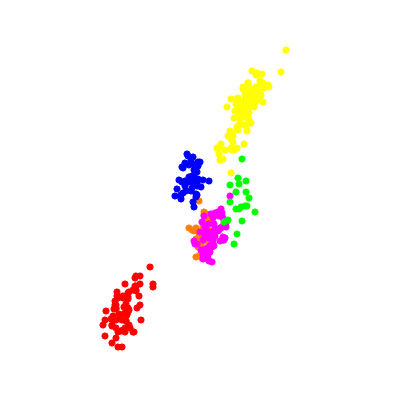
\includegraphics[width=0.5\textwidth]{img/der_freeviz.png}}
	\subfigure[MDS]{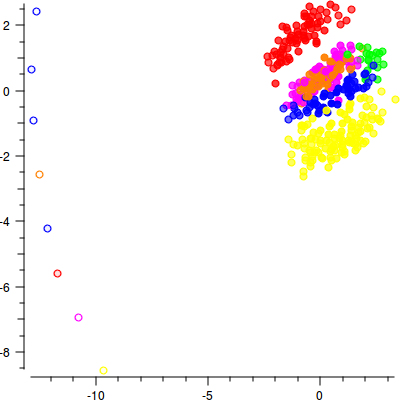
\includegraphics[width=0.5\textwidth]{img/der_mds.png}}
	\subfigure[uniclass]{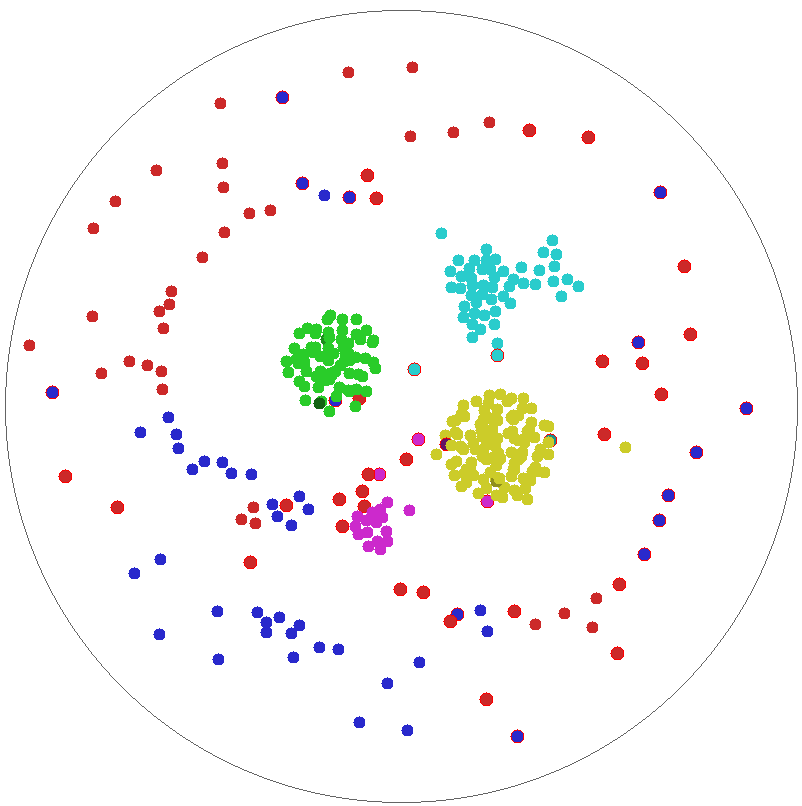
\includegraphics[width=0.6\textwidth]{img/der_uniclass.png}}
	\end{center}
	\caption{To je caption}
	\label{f-derm}
	\end{figure}
	
\section{Klasifikacija}

\section{Clustering}

\section{Zaklju"cek}
	
\end{document}
